\documentclass{../khlslides}


\title[Loops]{Loops}
\author{Fr\'ed\'eric Vogels}


\pgfkeys{/tikz/flowchart/node/.style={rectangle,fill=blue,opacity=0.5,text opacity=1,drop shadow,inner sep=2mm}}
\pgfkeys{/tikz/flowchart/arrow/.style={-latex,flowchart/arrowline}}
\pgfkeys{/tikz/flowchart/arrowline/.style={thick}}


\newcommand{\lcurly}{{\tt{\char '173}}}
\newcommand{\link}[2]{\href{#1}{\beamergotobutton{#2}}}
\newcommand{\PLACEHOLDER}[1]{\ensuremath{\langle}\textrm{\textit{#1}\ensuremath{\rangle}}}


\pgfkeys{
  /wof/sequence point/.cd,
  placement/.initial=above,
  /wof/sequence link/.cd,
  label/.initial={},
  /wof/round/.cd,
  name prefix/.initial=,
  /tikz/.cd,
  sequence point/.style={blue!50,thick,fill=white},
  sequence point label/.style={font=\tiny,black},
  sequence link/.style={blue!50,thick},
  active/.style={fill=red,thick,red}
}
\newcommand{\seqpoint}[3][]{{
  \pgfkeys{/wof/sequence point/.cd,#1}
  \pgfkeys{/wof/sequence point/placement/.get=\placement}
  \pgfkeys{/wof/round/name prefix/.get=\prefix}
  \draw[sequence point] (\prefix\space#2) circle (.05)
                        node[sequence point label,\placement] {#3};
}}
\newcommand{\seqlink}[3][]{{
  \pgfkeys{/wof/sequence link/.cd,#1}
  \pgfkeys{/wof/sequence link/label/.get=\seqlinklabel}
  \pgfkeys{/wof/round/name prefix/.get=\prefix}
  \draw[sequence link] (\prefix\space#2) -- (\prefix\space#3) node[midway,sloped,yshift=1mm,font=\tiny,black] {\seqlinklabel};
}}

\newcommand{\singleround}[1][]{{
  \pgfkeys{/wof/round/.cd,#1}
  \pgfkeys{/wof/round/name prefix/.get=\prefix}
  \def\COORD (##1) at ##2;{\coordinate (\prefix\space##1) at ##2;}

  \COORD (init) at (0,0);
  \COORD (turn wheel) at ($ (\prefix\space init) + (1,2) $);
  \COORD (bankruptcy lose money) at ($ (\prefix\space turn wheel) + (1,1.5) $);
  \COORD (bankruptcy next player) at ($ (\prefix\space bankruptcy lose money) + (2,0) $);
  \COORD (pass) at ($ (\prefix\space turn wheel) + (3,0.5) $);
  \COORD (joker) at ($ (\prefix\space turn wheel) + (3,-0.5) $);
  \COORD (consonant) at ($ (\prefix\space turn wheel) + (1,-2) $);
  \COORD (show consonant) at ($ (\prefix\space consonant) + (1,0) $);
  \COORD (gain) at ($ (\prefix\space show consonant) + (1,0.5) $);
  \COORD (no consonants) at ($ (\prefix\space show consonant) + (1,-0.5) $);
  \COORD (end consonants) at ($ (\prefix\space show consonant) + (2,0) $);
  \COORD (vowel) at ($ (\prefix\space init) + (1,-2) $);
  \COORD (buy vowel) at ($ (\prefix\space vowel) + (1.5,0) $);
  \COORD (show vowels) at ($ (\prefix\space buy vowel) + (1.5,0) $);
  \COORD (no vowels) at ($ (\prefix\space show vowels) + (1,.5) $);
  \COORD (end vowels) at ($ (\prefix\space show vowels) + (2,0) $);
  \COORD (exit) at ($ (\prefix\space init) + (8,0) $);

  \seqlink[label=rad]{init}{turn wheel}
  \seqlink[label=bankroet]{turn wheel}{bankruptcy lose money}
  \seqlink{bankruptcy lose money}{bankruptcy next player}
  \seqlink[label=verlies beurt]{turn wheel}{pass}
  \seqlink[label=joker]{turn wheel}{joker}
  \seqlink[label=else]{turn wheel}{consonant}
  \seqlink{consonant}{show consonant}
  \seqlink[label=0]{show consonant}{no consonants}
  \seqlink[label=1+]{show consonant}{gain}
  \seqlink{gain}{end consonants}
  \seqlink{no consonants}{end consonants}
  \seqlink{end consonants}{exit}
  \seqlink{joker}{exit}
  \seqlink{pass}{exit}
  \seqlink{bankruptcy next player}{exit}
  \seqlink[label=klinker]{init}{vowel}
  \seqlink{vowel}{buy vowel}
  \seqlink{buy vowel}{show vowels}
  \seqlink[label=0]{show vowels}{no vowels}
  \seqlink{no vowels}{end vowels}
  \seqlink[label=1+]{show vowels}{end vowels}
  \seqlink{end vowels}{exit}

  \seqpoint[placement=above left]{init}{rad/klinker}
  \seqpoint[placement=left]{turn wheel}{draai rad}
  \seqpoint{bankruptcy lose money}{score = 0}
  \seqpoint{bankruptcy next player}{huidigeSpeler++}
  \seqpoint{pass}{huidigeSpeler++}
  \seqpoint{joker}{jokers++}
  \seqpoint[placement=below]{consonant}{gok medeklinker}
  \seqpoint{show consonant}{toon}
  \seqpoint{gain}{score += bedrag * k}
  \seqpoint[placement=below]{no consonants}{huidigeSpeler++}
  \seqpoint{end consonants}{}
  \seqpoint[placement=below]{vowel}{gok klinker}
  \seqpoint[placement=below]{buy vowel}{score -= 50}
  \seqpoint[placement=below]{show vowels}{toon}
  \seqpoint{no vowels}{huidigeSpeler++}
  \seqpoint{end vowels}{}
  \seqpoint{exit}{}
}}


\begin{document}

\begin{frame}
  \titlepage
\end{frame}

\begin{frame}
  \frametitle{Basiselementen Algoritmes}
  \begin{center}
    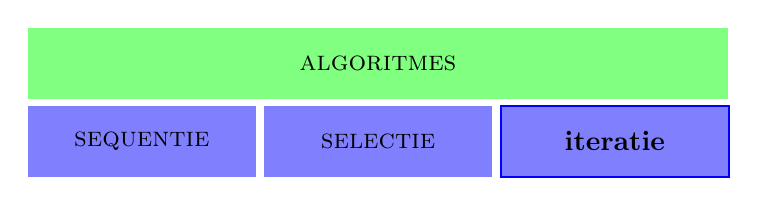
\begin{tikzpicture}[building block/.style={minimum width=2.9cm,minimum height=.9cm,fill=blue!50,font=\sc},
                        algorithm/.style={minimum width=8.9cm,minimum height=.9cm,fill=green!50,font=\sc}]
      \node[building block,anchor=south west] at (0,0) { sequentie };
      \node[building block,anchor=south west] at (3,0) { selectie };
      \node[building block,anchor=south west,draw=blue,thick] at (6,0) { \bfseries iteratie };
      \node[algorithm,anchor=south west] at (0,1) { algoritmes };
    \end{tikzpicture}
  \end{center}
\end{frame}

\begin{frame}
  \frametitle{Rad van Fortuin}
  \begin{center}
    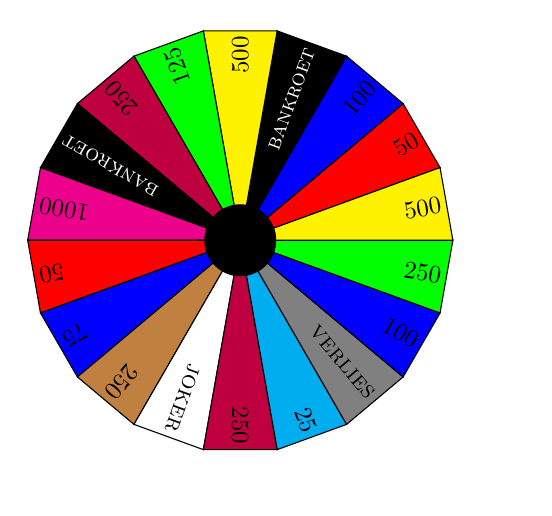
\begin{tikzpicture}[scale=.9,transform shape]
      \path[use as bounding box] (-3,-3.5) rectangle (4,3);

      \foreach[count=\i] \text/\c in {50/red,100/blue,{\color{white}\sc\small bankroet}/black,500/yellow,125/green,250/purple,{\color{white}\sc\small bankroet}/black,1000/magenta,50/red,75/blue,250/brown,{\sc joker}/white,250/purple,25/cyan,{\sc verlies}/gray,100/blue,250/green,500/yellow} {
        \pgfmathparse{20}\let\deltaangle\pgfmathresult
        \pgfmathparse{\i * \deltaangle}\let\startangle\pgfmathresult
        \pgfmathparse{\startangle + \deltaangle/2}\let\midangle\pgfmathresult
        \pgfmathparse{\startangle + \deltaangle}\let\endangle\pgfmathresult
        \draw[fill=\c] (0,0) -- (\startangle:3cm) -- (\endangle:3cm) -- cycle;
        \coordinate (cell \i) at (\midangle:3cm);
        \node[anchor=east,rotate=\midangle] at (\midangle:3cm) {\text};
      }
      \draw[fill=black] (0,0) circle (.5cm);
    \end{tikzpicture}
    \vskip4mm
    We herbezoeken hetzelfde voorbeeld
  \end{center}
\end{frame}



\begin{frame}
  \frametitle{Rad van Fortuin: E\'en Beurt}
  \begin{center}
    \begin{tikzpicture}
      \singleround
    \end{tikzpicture}
  \end{center}
\end{frame}

\begin{frame}
  \frametitle{Rad van Fortuin: Twee Beurten}
  \begin{center}
    \begin{tikzpicture}
      \begin{scope}[scale=0.5,transform shape]
        \singleround[name prefix=a]
      \end{scope}

      \begin{scope}[scale=0.5,transform shape,xshift=10cm]
        \singleround[name prefix=b]
      \end{scope}

      \draw[sequence link] (a exit) -- (b init);
    \end{tikzpicture}
  \end{center}
\end{frame}

\begin{frame}
  \frametitle{Rad van Fortuin: Drie Beurten}
  \begin{center}
    \begin{tikzpicture}
      \begin{scope}[scale=0.33,transform shape]
        \singleround[name prefix=a]
      \end{scope}

      \begin{scope}[scale=0.33,transform shape,xshift=10cm]
        \singleround[name prefix=b]
      \end{scope}

      \begin{scope}[scale=0.33,transform shape,xshift=20cm]
        \singleround[name prefix=c]
      \end{scope}

      \draw[sequence link] (a exit) -- (b init);
      \draw[sequence link] (b exit) -- (c init);
    \end{tikzpicture}
  \end{center}
\end{frame}

\begin{frame}
  \frametitle{Rad van Fortuin: 16 Beurten}
  \begin{center}
    \begin{tikzpicture}
      \begin{scope}[scale=0.20,transform shape]
        \singleround[name prefix=1]
      \end{scope}

      \begin{scope}[scale=0.20,transform shape,xshift=10cm]
        \singleround[name prefix=2]
      \end{scope}

      \begin{scope}[scale=0.20,transform shape,xshift=20cm]
        \singleround[name prefix=3]
      \end{scope}

      \begin{scope}[scale=0.20,transform shape,xshift=30cm]
        \singleround[name prefix=4]
      \end{scope}

      \begin{scope}[scale=0.20,transform shape,xshift=35cm,yshift=-6cm,rotate=180]
        \singleround[name prefix=5]
      \end{scope}

      \begin{scope}[scale=0.20,transform shape,xshift=25cm,yshift=-6cm,rotate=180]
        \singleround[name prefix=6]
      \end{scope}

      \begin{scope}[scale=0.20,transform shape,xshift=15cm,yshift=-6cm,rotate=180]
        \singleround[name prefix=7]
      \end{scope}

      \begin{scope}[scale=0.20,transform shape,xshift=5cm,yshift=-6cm,rotate=180]
        \singleround[name prefix=8]
      \end{scope}

      \begin{scope}[scale=0.20,transform shape,yshift=-15cm]
        \singleround[name prefix=9]
      \end{scope}

      \begin{scope}[scale=0.20,transform shape,xshift=10cm,yshift=-15cm]
        \singleround[name prefix=10]
      \end{scope}

      \begin{scope}[scale=0.20,transform shape,xshift=20cm,yshift=-15cm]
        \singleround[name prefix=11]
      \end{scope}

      \begin{scope}[scale=0.20,transform shape,xshift=30cm,yshift=-15cm]
        \singleround[name prefix=12]
      \end{scope}

      \begin{scope}[scale=0.20,transform shape,xshift=35cm,yshift=-21cm,rotate=180]
        \singleround[name prefix=13]
      \end{scope}

      \begin{scope}[scale=0.20,transform shape,xshift=25cm,yshift=-21cm,rotate=180]
        \singleround[name prefix=14]
      \end{scope}

      \begin{scope}[scale=0.20,transform shape,xshift=15cm,yshift=-21cm,rotate=180]
        \singleround[name prefix=15]
      \end{scope}

      \begin{scope}[scale=0.20,transform shape,xshift=5cm,yshift=-21cm,rotate=180]
        \singleround[name prefix=16]
      \end{scope}

      \foreach \i in {1,...,15} {
        \pgfmathparse{int(\i+1)}\let\j\pgfmathresult
        \draw[sequence link] (\i\space exit) |- (\j\space init);
      }
    \end{tikzpicture}
  \end{center}
\end{frame}

\begin{frame}
  \frametitle{Lus}
  \begin{center}
    \begin{tikzpicture}
      \path[use as bounding box] (0,-3) rectangle (8,4);
      \singleround[name prefix=b]
      \only<1-2>{
        \draw[sequence link,-latex,red] (b exit) -- +(0,-3) -| ($ (b init) + (0,-.2) $);
      }

      \only<3->{
        \draw[sequence link,-latex,red] (b exit) -- +(0,-3) node[midway,sloped,black,yshift=1mm,font=\tiny] {!spel gedaan} -| ($ (b init) + (0,-.2) $);
        \draw[sequence link,-latex,red] (b exit) -- +(2,0) node[midway,sloped,black,yshift=1mm,font=\tiny] {spel gedaan};
      }

      \only<2>{
        \node[opacity=.85,text opacity=1,fill=blue!50] (note) at (6,0) {\parbox{3cm}{\raggedright Lus laat toe berekeningen te herhalen}};
        \draw[-latex,blue!50,thick] (note) -- ($ (b exit) + (-0.1,-1) $);
      }

      \only<4>{
        \node[opacity=.85,text opacity=1,fill=blue!50] (note) at (8,2) {\parbox{3cm}{\raggedright Lus moet ooit eindigen}};
        \draw[-latex,blue!50,thick] (note) -- ($ (b exit) + (1,.2) $);
      }
    \end{tikzpicture}
  \end{center}
\end{frame}

%%% Local Variables: 
%%% mode: latex
%%% TeX-master: "loops"
%%% End: 

\begin{frame}
  \frametitle{Lussen in JavaScript}
  \begin{columns}
    \column{.5\linewidth}
    \begin{center}
      \begin{tikzpicture}
        \node[flowchart/node] (while) {evalueren \PLACEHOLDER{conditie}};
        \node (loop entry) at ($ (while.north) + (0,0.5) $) {};
        \node[flowchart/node] (body) at ($ (while.south) + (2,-2) $) {\parbox{1.5cm}{\centering uitvoeren \PLACEHOLDER{body}}};
        \node (split) at ($ (while.south) + (0,-0.5) $) {};

        \draw[flowchart/arrow] ($ (while.north) + (0,1) $) -- (while.north);
        \draw[flowchart/arrow] (while.south) -- (split.center) -- ++(-2,-0.5) -- ++(0,-2.5);
        \draw[flowchart/arrow] (split.center) -- ++(2,-0.5) -- (body.north);
        \draw[flowchart/arrowline] (body.south) -- ++(0,-0.5) -- ++(1.5,0) |- (loop entry.center);

        \path ($ (while.south) + (0,-0.4) $) -- ++(-2,-0.5) node [midway,above,sloped] {false};
        \path ($ (while.south) + (0,-0.4) $) -- ++(2,-0.5) node [midway,above,sloped] {true};
      \end{tikzpicture}
    \end{center}

    \column{.5\linewidth}
    \code{while.js}
  \end{columns}
\end{frame}

\begin{frame}
  \frametitle{Oefening}
  \code[width=.4\linewidth]{exwhile.js}

  \begin{center}
    \begin{tikzpicture}
      \coordinate (sp x init) at (0,0);
      \coordinate (sp i init) at ($ (sp x init) + (1.5,0) $);
      \coordinate (sp i check) at ($ (sp i init) + (1.5,0) $);
      \coordinate (sp x mul 2) at ($ (sp i check) + (1.5,-1) $);
      \coordinate (sp i dec) at ($ (sp x mul 2) + (1.5,0) $);
      \coordinate (sp exit) at ($ (sp i check) + (1.5,0) $);

      \visible<2->{
        \draw[sequence link] (sp x init) -- (sp i init);
        \draw[sequence link] (sp i init) -- (sp i check);
        \draw[sequence link] (sp i check) -- (sp x mul 2) node[midway,black,font=\tiny,sloped,yshift=1mm] {\tt true};
        \draw[sequence link] (sp x mul 2) -- (sp i dec);
        \draw[sequence link,-latex] (sp i dec) -- ++(0,-.5) -| (sp i check);
        \draw[sequence link] (sp i check) -- (sp exit) node[midway,black,font=\tiny,sloped,yshift=1mm] {\tt false};

        \draw[sequence point] (sp x init) circle (.05) node[above,font=\tiny,black] {\tt var x=1};
        \draw[sequence point] (sp i init) circle (.05) node[above,font=\tiny,black] {\tt var i = 5};
        \draw[sequence point] (sp i check) circle (.05) node[above,font=\tiny,black] {\tt i > 0};
        \draw[sequence point] (sp x mul 2) circle (.05) node[above right,font=\tiny,black] {\tt x *= 2};
        \draw[sequence point] (sp i dec) circle (.05) node[above,font=\tiny,black] {\tt i--};
        \draw[sequence point] (sp exit) circle (.05);

        \node[anchor=north west,font=\small] at ($ (sp x init) + (0,-1) $) {
          \begin{tabular}{c@{\hspace{1mm}}c@{\hspace{1mm}}l}
            x & = & \tt
            \only<2-4>{1}%
            \only<5-7>{2}%
            \only<8-10>{4}%
            \only<11-13>{8}%
            \only<14-16>{16}%
            \only<17->{32}%
            \\
            \only<3->{i} & \only<3->{=} & \tt
            \only<3-5>{5}%
            \only<6-8>{4}%
            \only<9-11>{3}%
            \only<12-14>{2}%
            \only<15-17>{1}%
            \only<18->{0}%
            \\
          \end{tabular}
        };

        \only<2>{
          \draw[active] (sp x init) circle (.05);
        }

        \only<3>{
          \draw[active] (sp i init) circle (.05);
        }

        \only<4,7,10,13,16,19>{
          \draw[active] (sp i check) circle (.05);
        }

        \only<5,8,11,14,17>{
          \draw[active] (sp x mul 2) circle (.05);
        }

        \only<6,9,12,15,18>{
          \draw[active] (sp i dec) circle (.05);
        }

        \only<20>{
          \draw[active] (sp exit) circle (.05);
        }
      }
    \end{tikzpicture}
  \end{center}
\end{frame}


%%% Local Variables: 
%%% mode: latex
%%% TeX-master: "loops"
%%% End: 


\begin{frame}
  \frametitle{Vaak Voorkomend Patroon}
  \code[width=.4\linewidth]{while-pattern.js}
  \begin{tikzpicture}[overlay,remember picture]
    \node[/khl/note] (note init) at ($ (init) + (0,1) $) {Initialisatie iterator};
    \draw[/khl/note arrow] (note init) -- (init);

    \node[/khl/note] (note cond) at ($ (cond) + (1,1) $) {Conditie};
    \draw[/khl/note arrow] (note cond) -- (cond);

    \node[/khl/note,anchor=west] (note inc) at ($ (inc) + (1,0) $) {Incrementatie};
    \draw[/khl/note arrow] (note inc) -- (inc);
  \end{tikzpicture}
\end{frame}

\begin{frame}
  \frametitle{For-lus}
  \begin{center}
    \code[width=.6\linewidth]{while-pattern2.js}
    \vskip2mm
    is equivalent met
    \vskip2mm
    \code[width=.6\linewidth]{for.js}
  \end{center}
\end{frame}

\begin{frame}
  \begin{columns}
    \column{.5\linewidth}
    \begin{tikzpicture}
      \node[flowchart/node] (init) {evalueren \PLACEHOLDER{init}};
      \node (loop) at ($ (init.south) + (0,-0.25) $) {};
      \node[flowchart/node] (cond) at ($ (init.south) + (0,-1) $) {evalueren \PLACEHOLDER{cond}};
      \node (split) at ($ (cond.south) + (0,-0.5) $) {};
      \node[flowchart/node] (body) at ($ (split.center) + (2,-1.5) $) {evalueren \PLACEHOLDER{body}};
      \node[flowchart/node] (inc) at ($ (body.south) + (0,-1) $) {evalueren \PLACEHOLDER{inc}};

      \draw[flowchart/arrow] ($ (init.north) + (0,0.5) $) -- (init.north);
      \draw[flowchart/arrow] (init.south) -- (cond.north);
      \draw[flowchart/arrow] (cond.south) -- (split.center) -- ++(-2,-0.5) -- ++(0,-3.5);
      \draw[flowchart/arrow] (split.center) -- ++(2,-0.5) -- (body.north);
      \draw[flowchart/arrow] (body.south) -- (inc.north);
      \draw[flowchart/arrowline] (inc.south) -- ++(0,-0.5) -- ++(2,0) |- (loop.center);

      \path ($ (split.center) + (0,.1) $) -- ++(-2,-0.5) node[midway,sloped,above] {\tt\tiny false};
      \path ($ (split.center) + (0,.1) $) -- ++(2,-0.5) node[midway,sloped,above] {\tt\tiny true};
    \end{tikzpicture}
    \column{.5\linewidth}
    \code[font size=\scriptsize]{for.js}
  \end{columns}
\end{frame}

\begin{frame}
  \frametitle{Oefening}
  \begin{center}
    Wat berekent de volgende code?
  \end{center}
  \code[width=.7\linewidth]{ex-for.js}
  \visible<2>{
    \begin{center}
      \tt j = 1 + 2 + 3 + 4 + 5 = 15
    \end{center}
  }
\end{frame}

\begin{frame}
  \frametitle{Keuze tussen {\tt while} en {\tt for}}
  \begin{itemize}
    \item {\tt while} en {\tt for} zijn even krachtig
          \begin{itemize}
            \item Een {\tt for}-lus kan als {\tt while}-lus herschreven worden
            \item Een {\tt while}-lus kan als {\tt for}-lus herschreven worden
          \end{itemize}
    \item Keuze kwestie van leesbaarheid
    \item Lus kiezen die best intentie weerspiegelt
    \item Gebruik {\tt for} indien
          \begin{itemize}
            \item er \'e\'en duidelijke iterator is, en
            \item deze enkel nuttig is binnen de lus, en
            \item deze bij elke stap verhoogd wordt
          \end{itemize}
  \end{itemize}
\end{frame}

\begin{frame}
  \frametitle{Oefening}
  Stel dat de variabele {\tt x} een positief geheel getal bevat. Schrijf code die berekent hoeveel opeenvolgende veelvouden van 3 je moet optellen
  opdat de som net kleiner dan het gegeven getal zou zijn. Schrijf dit aantal naar een variabele {\tt y}.

  \vskip5mm

  \structure{Voorbeeld} \\
  Bij {\tt x = 20} moet {\tt y === 3} want $3+6+9 = 18 \leq 20$ en $3+6+9+12 > 20$.
\end{frame}

\end{document}

%%% Local Variables: 
%%% mode: latex
%%% TeX-master: t
%%% End: 
